\section{Decimoctava iteración de la Fase 5: sistema de pruebas}
\label{sec:F5I18}

Ha sido un error no hacer de esta la primera iteración de la primera fase, ya que la práctica actual de la programación recomienda construir el sistema de pruebas antes siquiera de empezar con el código. Se han probado manualmente cada iteración siempre, y se han ido incluyendo pruebas automáticas a lo largo del desarrollo lanzadas de forma manual.

Esta iteración incluye las pruebas dentro del sistema, para que se puedan lanzar de manera más sencilla desde el propio \emph{Index.html}. Aquí se documenta cómo incluir el manejo de las pruebas en el diseñador y por qué. Los procesos para las pruebas en sí se fueron añadiendo principalmente a lo largo de las iteraciones anteriores (F5-I13 a F5-I17), usando algunos botones sueltos y varios scripts de Node. Aquí se unifica todo en una nueva pestaña \emph{Pruebas} que los incluye, se describe cómo se lanza, qué cubre y cómo se añade una prueba nueva.

\subsection{Principios}
\label{sec:F5I18Principios}

\begin{enumerate}
	\item \textbf{Una prueba, un sitio.} La lógica de cada prueba vive en un único fichero. Cambiar una prueba no obliga a tocar nada más.

	\item \textbf{Dos formas de lanzarla, un solo código.} Un botón en la pestaña \emph{Pruebas} y un comando de consola ejecutan exactamente la misma función. El comando no contiene pruebas: abre la página con un navegador automático y llama a la misma función que el botón.

	\item \textbf{Solo es público lo que otros módulos necesitan.} Ninguna función se hace pública por comodidad de las pruebas. Lo que no se puede probar desde fuera se prueba en una copia temporal (ver~\ref{sec:F5I18Editor}).

	\item \textbf{Sin depender de cartuchos ajenos.} Para que las pruebas tengan sentido usan sus propios cartuchos, que han sido copiados a \texttt{pruebas/cartuchos}, o bien cartuchos de laboratorio construidos en memoria, de modo que regenerar los cartuchos de ejemplo del proyecto no las rompe.

	\item \textbf{Un resultado inequívoco.} Cada lanzamiento termina en una línea \texttt{RESULTADO: OK} o \texttt{RESULTADO: ERROR (detalle)} y con código de salida 0 o 1.

	\item \textbf{Reproducir antes de corregir.} Una prueba nueva debe fallar con el código anterior (criterio de F5-I15).
	
	\item \textbf{Reproducible}: Las pruebas se pueden lanzar sin problema varias veces, por lo que tras cada iteración se realizará una prueba completa para asegurarnos de que todo sigue funcionando.
	
\end{enumerate}

\subsection{Arquitectura}
\label{sec:F5I18Arquitectura}

\begin{itemize}
	\item \texttt{pruebas/pruebas.js} es el \textbf{ejecutor}. Guarda el catálogo de pruebas (\texttt{registrar}), crea los botones y el panel «Desde consola» (\texttt{inicializar}) y ofrece \texttt{ejecutar(id)} para el lanzador. También reúne las utilidades que comparten las pruebas (\texttt{util}): comparaciones, espera, lectura de ficheros del proyecto por URL, entrega de ficheros a los inputs del diseñador, cartucho de laboratorio y CRC independiente.
	\item Cada fichero \texttt{pruebas*.js} \textbf{registra} sus pruebas en el catálogo. Una prueba es un objeto con \texttt{id}, \texttt{grupo}, \texttt{nombre}, \texttt{ejecutar(opciones)} y, si procede, \texttt{necesita} (por ejemplo, un GWI cargado), \texttt{destructiva} (sustituye el cartucho cargado) y \texttt{soloConsola} (sin botón). \texttt{ejecutar} devuelve una lista \texttt{[nombre, ok, detalle]}, o \texttt{null} si faltan los datos que necesita, lo que se muestra como aviso y no como fallo.
	\item \texttt{pruebas/lanzador.js} es el \textbf{lanzador de consola}: sirve el proyecto por http en el propio equipo, abre \texttt{index.html} con Playwright, ejecuta en la página las pruebas del grupo y las escribe por consola. Cualquier excepción (Playwright sin instalar, navegador que no arranca) acaba también como \texttt{RESULTADO: ERROR}.
	\item \texttt{pruebas/servidor.js} sirve la raíz del proyecto y abre \texttt{index.html} en el navegador (ver~\ref{sec:F5I18Servidor}). Comparte el servidor con el lanzador.
\end{itemize}

\subsection{Grupos de pruebas y códigos}
\label{sec:F5I18Grupos}

Cada prueba lleva un código (M, D, E, G, C, T) que aparece en el botón y en el informe, para poder citarla. Las pruebas que cargan cartuchos propios sustituyen el cartucho cargado en el diseñador: el botón lo avisa y hay que volver a cargarlo después.

\begin{table}[H]
	\centering
	\begin{tabularx}{\textwidth}{l >{\RaggedRight\arraybackslash}X >{\RaggedRight\arraybackslash}p{2.3cm}}
		\toprule
		\textbf{Fichero} & \textbf{Códigos y qué prueba} & \textbf{Botón} \\
		\midrule
		\texttt{pruebasMotor.js} & \textbf{M0--M5.} Motor de estados: orden del tick, secundarios, iconos, barrido, colisión, secuencia y congelación, jugador. Montan su cartucho en memoria y dejan las listas del motor como estaban & Sí \\
		\midrule
		\texttt{pruebasDirector.js} & \textbf{D1--D9.} Carga de cartuchos: GWC sin máquina (F5-I19, página recién cargada), carga sin setup, cambio de máquina en caliente y botón «Limpiar» de la Carga (F5-I19), GWC tras GWI, cartucho incompatible, GWB que no descompone y aviso del historial descartado al cargar un GWB sobre una autoría; aplicar/cargar un setup propaga los datos comunes a la ficha de Cartucho y pide confirmación antes de descartar (F5-I20) & D5 no; el resto (destructivas) \\
		\midrule
		\texttt{pruebasEditor.js} & \textbf{E1--E9.} Editor: historial, ids de las piezas de unión, deshacer y rehacer, cambio de tipo, numeración, uniones, PNG con alfa y verificación & No \\
		\midrule
		\texttt{pruebasGenerales.js} & \textbf{G1--G3.} Formato GWC (CRC y lector) y \texttt{ColorFondo}, en el GWC y en la ficha y el GWB & Sí (G3 destructiva) \\
		\midrule
		\texttt{pruebasGWI\_GWC.js} & \textbf{C1--C8.} Equivalencia entre el GWI y el GWC que sale de él (datos y partidas tick a tick), y el par GWI/GWC: \texttt{codigoGWC} de la ficha, guardar que lo desparea, generar desfasado y el porcentaje de memoria indicado al generar (F5-I20) & Sí (C3 y C4 destructivas) \\
		\midrule
		\texttt{pruebasTeclas.js} & \textbf{T1--T3.} Teclas del simulador: cursores, rechazos, teclas por defecto de cada estilo y teclas propias del cartucho, con la precedencia GWI $>$ GWB $>$ GWS; el dígito 1/2/3 solo como tecla en el trío A/B/R (F5-I17, M6/M7/M8) & Sí (destructivas) \\
		\bottomrule
	\end{tabularx}
	\caption{Grupos de pruebas.}
\end{table}


\subsection{Cómo se lanzan}
\label{sec:F5I18Lanzar}

\textbf{Desde la pestaña.} \texttt{index.html} se abre por servidor local (ver~\ref{sec:F5I18Servidor}) con \texttt{GW\_DEBUG} activo. La pestaña \emph{Pruebas} muestra un botón por prueba, agrupadas, y debajo el panel \emph{Desde consola}: una línea por grupo, con su código S1--S7, el comando que lo lanza y un botón \emph{Copiar}.

\begin{figure}[H]
	\centering
	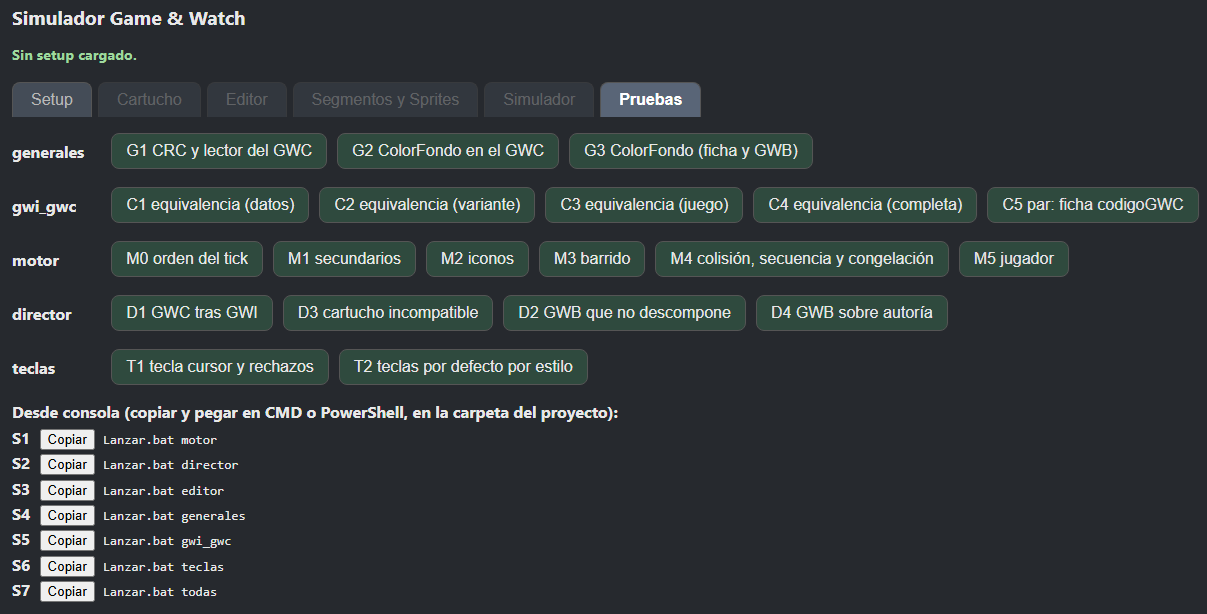
\includegraphics[width=0.60\linewidth]{imagenes/Propias/C05-I029}
	\caption[Resultado de las pruebas]{Resultado de las pruebas}
	\label{fig:c05-i029}
\end{figure}

\textbf{Desde la consola (Windows).} Se copia una línea del panel y se pega en CMD o PowerShell, parado en la carpeta \texttt{pruebas} del proyecto (donde está \texttt{Lanzar.bat}; también funciona desde cualquier otra carpeta poniendo la suya delante, \texttt{pruebas\textbackslash Lanzar.bat motor}, porque el \texttt{.bat} localiza sus propias rutas):

\begin{itemize}
	\item \texttt{S1}: \texttt{Lanzar.bat motor}; \texttt{S2}: \texttt{director}; \texttt{S3}: \texttt{editor}; \texttt{S4}: \texttt{generales}; \texttt{S5}: \texttt{gwi\_gwc}; \texttt{S6}: \texttt{teclas}.
	\item \texttt{S7}: \texttt{Lanzar.bat todas}: las lanza todas, una detrás de otra, y escribe un resumen por grupo. Tarda unos minutos, sobre todo por las partidas de GWI/GWC.
\end{itemize}

\textbf{Botones y scripts.} Los scripts cubren todas las pruebas, también las que no tienen botón:

\begin{itemize}
	\item \textbf{Con botón en la pestaña} (y también por script): motor (M0--M5, S1), director (D1--D9, S2; D5 exige página recién cargada y es la primera de la suite), generales (G1--G3, S4; G3 destructiva), gwi\_gwc C1--C5 (S5; C3 y C4 destructivas, C1, C2 y C5 necesitan un GWI cargado) y teclas (T1--T3, S6; destructivas).
	\item \textbf{Solo por script} (\texttt{soloConsola}, sin botón; necesitan un GWI cargado): editor (E1--E9, S3) y gwi\_gwc C6--C8 (S5).
\end{itemize}

\texttt{Lanzar.bat} recibe el nombre del grupo (sin parámetro, o con uno desconocido, muestra la ayuda) y llama al script de PowerShell correspondiente (\texttt{pruebasMotor.ps1} y los demás; \texttt{pruebasTodas.ps1} los encadena). Todos cargan primero \texttt{\_preparar.ps1}, que comprueba que Node.js esté instalado, instala Playwright de forma global si falta (\texttt{npm i -g playwright}), define \texttt{NODE\_PATH} con la carpeta global de npm y descarga el navegador. La primera vez tarda. \texttt{Lanzar.bat} arranca PowerShell con \texttt{-ExecutionPolicy Bypass}, de modo que no hace falta cambiar la política de scripts. Los \texttt{.bat} y los \texttt{.ps1} se guardan con fin de línea CRLF (\texttt{.gitattributes}).

\textbf{Opciones} (variables de entorno, por ejemplo \verb|$env:SEMILLAS="1,6699"| en PowerShell), para las pruebas de juego de GWI/GWC:

\begin{itemize}
	\item \texttt{SEMILLAS}, \texttt{TICKS} y \texttt{SIN\_PULSAR}: semillas jugadas (cinco por defecto), número de ticks y partida sin pulsaciones.
	\item \texttt{GRABAR=fichero}: guarda las partidas jugadas.
	\item \texttt{COMPARAR=fichero}: las compara con las guardadas. Es la red de seguridad del motor (criterio 2 de F5-I15).
\end{itemize}

\begin{figure}[H]
	\centering
	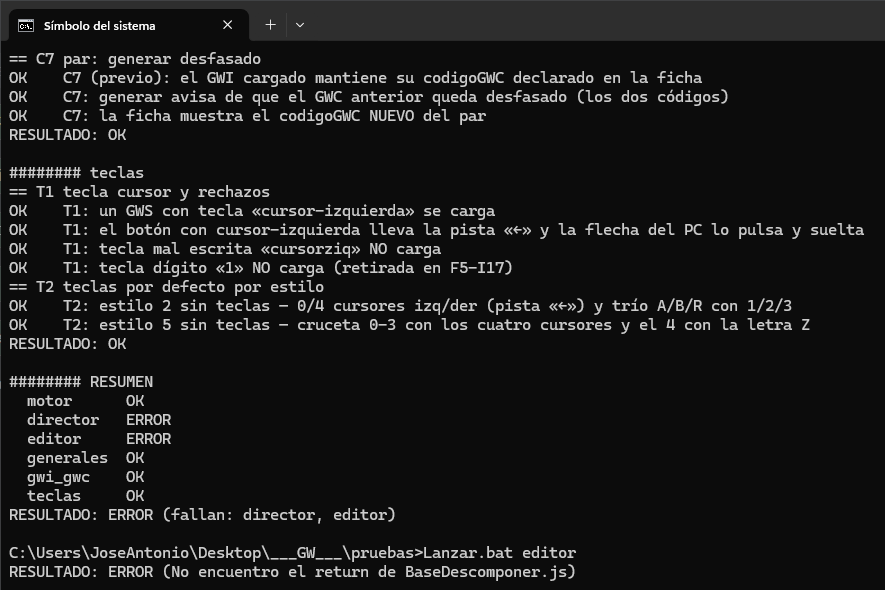
\includegraphics[width=0.60\linewidth]{imagenes/Propias/C05-I028}
	\caption[Resultado de las pruebas]{Resultado de las pruebas}
	\label{fig:c05-i028}
\end{figure}

\subsection{Servidor local}
\label{sec:F5I18Servidor}

Las pruebas que cargan cartuchos propios los leen del proyecto por URL. Con \texttt{index.html} abierto con doble clic (\texttt{file://}) el navegador lo bloquea y la prueba falla con «No se pudo leer \ldots{} (Failed to fetch)». Por eso \texttt{index.html} debe abrirse siempre por http. \texttt{pruebas\textbackslash Servidor.bat [puerto]} (o \texttt{node pruebas/servidor.js}) sirve la raíz del proyecto solo en el propio equipo (127.0.0.1), prueba los puertos siguientes si el 8080 está ocupado y abre el navegador en la dirección. Si \texttt{node} no está en el PATH, el \texttt{.bat} lo busca en las ubicaciones de instalación habituales. Para parar se pulsa Ctrl+C. El lanzador de consola no lo necesita: arranca su propio servidor.

\subsection{El Editor: pruebas solo de consola}
\label{sec:F5I18Editor}

Las pruebas del Editor necesitan ver el interior de \texttt{BaseDescomponer}, que vive dentro de una función cerrada, y el código de producción no lo publica. Para ellas el lanzador sirve una \emph{copia temporal} del proyecto en la que \texttt{BaseDescomponer.js} exporta además un objeto \texttt{\_t} con los interiores que lista \texttt{pruebasEditor.js}. El resto del sistema es el mismo: la prueba está registrada, se ejecuta dentro de la página y devuelve los mismos resultados. En la pestaña real esa prueba no tiene botón (\texttt{soloConsola}); si se llama desde ella, responde que solo se lanza desde la consola.

\subsection{Cartuchos de las pruebas}
\label{sec:F5I18Cartuchos}

Los cartuchos están en \texttt{pruebas/cartuchos}: \texttt{setup2.json}, \texttt{setup4.json} y \texttt{setup5.json}, \texttt{cartucho\_GWI.zip}, \texttt{cartucho\_GWB.zip} y \texttt{cartucho.GWC}. Las variantes que hacen falta (un GWB con otro nombre, un botón inexistente o la imagen \texttt{img\_s} en blanco; un GWI con rutas, aceleración y pausas declaradas) se construyen en memoria con JSZip a partir de ellos. Las pruebas del formato GWC usan además un cartucho de laboratorio de tres segmentos, porque algunas corrompen bytes concretos del fichero para comprobar el CRC y los errores del lector; su resolución es la menor que admite el GWC.

\textbf{Prueba de juego.} La partida del GWI y la del GWC se juegan dentro de la página sustituyendo temporalmente el reloj (\texttt{setTimeout}) por una cola que se vacía a mano, con un jugador determinista y la misma semilla. Se compara, tick a tick, qué segmentos están encendidos. Al terminar se restaura el reloj y se vuelve a cargar el GWI de ejemplo.

\subsection{Incidencias al montar el sistema}
\label{sec:F5I18Incidencias}

\begin{table}[H]
	\centering
	\begin{tabularx}{\textwidth}{l >{\RaggedRight\arraybackslash}X >{\RaggedRight\arraybackslash}X}
		\toprule
		\textbf{\#} & \textbf{Qué pasó} & \textbf{Solución} \\
		\midrule
		1 & Las pruebas de GWC fallaban con «la resolución 100$\times$80 está fuera del rango de pantallas (320$\times$240 a 1024$\times$600)»: el cartucho de laboratorio era anterior a la regla de F5-I16/F5-I17 & El cartucho de laboratorio pasa a 320$\times$240, la menor resolución admitida \\
		2 & Con \texttt{index.html} abierto por \texttt{file://} las pruebas que leen cartuchos fallaban con «Failed to fetch» y sin más pista & El mensaje incluye ahora el código HTTP y la dirección desde la que se lanza; \texttt{Servidor.bat} arranca el servidor local \\
		3 & D4 fallaba: el aviso «se descarta el historial» no salía nunca al cargar un GWB sobre una autoría. El número de acciones se contaba después de que la limpieza del cartucho reseteara la autoría, es decir, siempre valía 0 & Es un fallo del código, no de la prueba: las acciones se cuentan antes de limpiar (\texttt{BaseDirector.js}) \\
		4 & Un \texttt{.gitattributes} con una coma sobrante en la línea de los \texttt{.ps1} dejaba sin efecto el fin de línea CRLF de esos ficheros & Quitar la coma. Dentro del repositorio los ficheros se guardan normalizados (LF) y en la carpeta de trabajo salen con CRLF \\
		5 & La copia temporal del Editor se hacía con \texttt{cp -r}, que no existe en Windows & Se hace con \texttt{fs.cpSync} de Node, sin las carpetas de la memoria ni de Git \\
		\bottomrule
	\end{tabularx}
	\caption{Incidencias y soluciones.}
\end{table}

La incidencia 3 muestra el valor del sistema: D4 comprueba el aviso con un cartucho real y destapó un fallo que no daba ninguna señal al usar el diseñador a mano.

\subsection{Cómo añadir una prueba}
\label{sec:F5I18Nueva}

\begin{enumerate}
	\item Escribir la función en el fichero de su grupo (o crear un fichero nuevo \texttt{pruebas*.js}). Devuelve \texttt{[[nombre, ok, detalle], \ldots]}. Los nombres de las funciones propias del módulo llevan el prefijo \texttt{\_}.
	\item Registrarla con \texttt{Pruebas.registrar}: \texttt{id}, \texttt{grupo}, \texttt{nombre} (con su código), y \texttt{necesita}, \texttt{destructiva} o \texttt{soloConsola} si procede.
	\item Si es un fichero nuevo: cargarlo en \texttt{index.html} después de \texttt{pruebas.js}, y añadir el script \texttt{.ps1} y la línea correspondiente de \texttt{Lanzar.bat} y de \texttt{pruebasTodas.ps1}.
	\item Comprobar que \textbf{falla} con el código sin corregir y pasa con el corregido.
	\item Actualizar la cabecera del fichero (lista de funciones), el \texttt{README.md} y esta sección.
\end{enumerate}

\subsection{Ficheros del sistema}
\label{sec:F5I18Ficheros}

\begin{itemize}
	\item \texttt{pruebas/pruebas.js}, \texttt{lanzador.js} y \texttt{servidor.js}.
	\item \texttt{pruebas/pruebasMotor.js}, \texttt{pruebasDirector.js}, \texttt{pruebasEditor.js}, \texttt{pruebasGenerales.js}, \texttt{pruebasGWI\_GWC.js} y \texttt{pruebasTeclas.js}.
	\item \texttt{pruebas/Lanzar.bat}, \texttt{Servidor.bat}, \texttt{\_preparar.ps1}, un \texttt{.ps1} por grupo y \texttt{pruebasTodas.ps1}.
	\item \texttt{pruebas/cartuchos/}.
	\item \texttt{index.html} (carga de los ficheros de pruebas), \texttt{.gitattributes} y \texttt{README.md}.
\end{itemize}

\subsection{Estado}
\label{sec:F5I18Estado}

Con los cartuchos de \texttt{pruebas/cartuchos} y el código de F5-I17 con el fallo de la incidencia 3 corregido, los seis grupos (motor, director, editor, generales, gwi\_gwc y teclas) terminan en \texttt{RESULTADO: OK} al lanzarlos por el lanzador de consola con Node y Playwright.